\documentclass[12pt, oneside, a4paper]{scrreprt}
\usepackage[manualmark,headsepline,footsepline]{scrlayer-scrpage}

\usepackage[german]{babel}
\usepackage[utf8]{inputenc}
\usepackage{graphicx} %Grafik aktivieren
\usepackage{float}
\usepackage[final]{pdfpages}
\usepackage{hyperref}
\usepackage{pdfcomment}

\usepackage{siunitx}  
\sisetup{locale = DE,separate-uncertainty}  

\usepackage[backend=biber]{biblatex}
\addbibresource{xmpl.bib}


%% used for pgfplots, tikzpicture
\usepackage{pgfplots}
\pgfplotsset{compat=newest}

%% the following commands are needed for some matlab2tikz features
\usetikzlibrary{plotmarks}
\usetikzlibrary{arrows.meta}
\usepgfplotslibrary{patchplots}
\usepackage{grffile}
\usepackage{amsmath}

\pgfplotsset{plot coordinates/math parser=false}
\newlength\fwidth
  
%%%%%%%%%%%%%%%%%%%%%%%%%%%%%%%%%%%%%%%%%%%%%%%%

%Kapitel-Layout
\usepackage{lmodern} 
\usepackage{xcolor}
\colorlet{chapter}{black!75}
\addtokomafont{chapter}{\color{chapter}}
\makeatletter% siehe De-TeX-FAQ
\renewcommand*{\chapterformat}{%
  \begingroup% damit \unitlength-Änderung lokal bleibt 
  \setlength{\unitlength}{1mm}% 
  \begin{picture}(20,20)(0,5)% 
  \setlength{\fboxsep}{0pt}% 
  \put(20,20){\line(1,0){\dimexpr 
  \textwidth-20\unitlength\relax\@gobble}}% 
  \put(0,0){\makebox(15,20)[r]{% 
  \fontsize{18\unitlength}{28\unitlength}\selectfont\thechapter 
  \kern-.04em% Ziffer in der Zeichenzelle nach rechts schieben 
  }}% 
  \end{picture} % <-- Leerzeichen ist hier beabsichtigt! 
  \newline
  \endgroup
}

\setlength\parindent{0pt}

%%%%%%%%%%%%%%%%%%%%%%%%%%%%%%%%%%%%%%%%%%%%%%%%

% Kopf- und Fußzeilen, Seitenränder etc.
% Kopf- und Fußzeilen ------------------------------------------------------
\pagestyle{scrheadings}

% Kopf- und Fußzeile auch auf Kapitelanfangsseiten -------------------------
\renewcommand*{\chapterpagestyle}{scrheadings}

% Schriftform der Kopfzeile ------------------------------------------------
\renewcommand{\headfont}{%
\normalfont
}

% Kopfzeile ----------------------------------------------------------------
\ihead{Regelungstechnisches Praktikum (RTP)}
\chead{}
\ohead{
\includegraphics[width=0.3\textwidth]{Bilder/oth-regensburg-logo}}
%
\setlength{\headheight}{21mm} % Höhe der Kopfzeile
\setheadsepline[text]{0.4pt} % Trennlinie unter Kopfzeile

% Fußzeile -----------------------------------------------------------------
\ifoot{Torsten Reitmeier/Klaus Falkner}
\cfoot{\today}
\ofoot{\pagemark}


% erzeugt ein wenig mehr Platz hinter einem Punkt --------------------------
\frenchspacing 

\clubpenalty = 10000
\widowpenalty = 10000 
\displaywidowpenalty = 10000

\newcommand{\mt}[1]{\textrm{#1}}

%%%%%%%%%%%%%%%%%%%%%%%%%%%%%%%%%%%%%%%%%%%%%%%%

\begin{document}

 \begin{titlepage}

	\begin{tabular}{l r} 
 
      
\includegraphics[width=0.4\textwidth]{Bilder/oth-regensburg-logo}
      &
		
   \end{tabular}


   \begin{minipage} [c] [8.5cm] [b] {\textwidth}
      \Huge{
         \begin{center}
            \textbf{Praktikum Regelungstechnik (RTP)}\\[0.8cm]
             \par
              {\large Versuch 100:}\\[1cm]
              {\large Parameterbestimmung der Pumpzelle einer Lambdasonde\\ zur Vorbereitung der Reglerauslegung} \\[1cm]
          \end{center}
           }
      
   \end{minipage}

 \vspace{0.1cm}
 
   \begin{figure}[H]
	   \centering
		  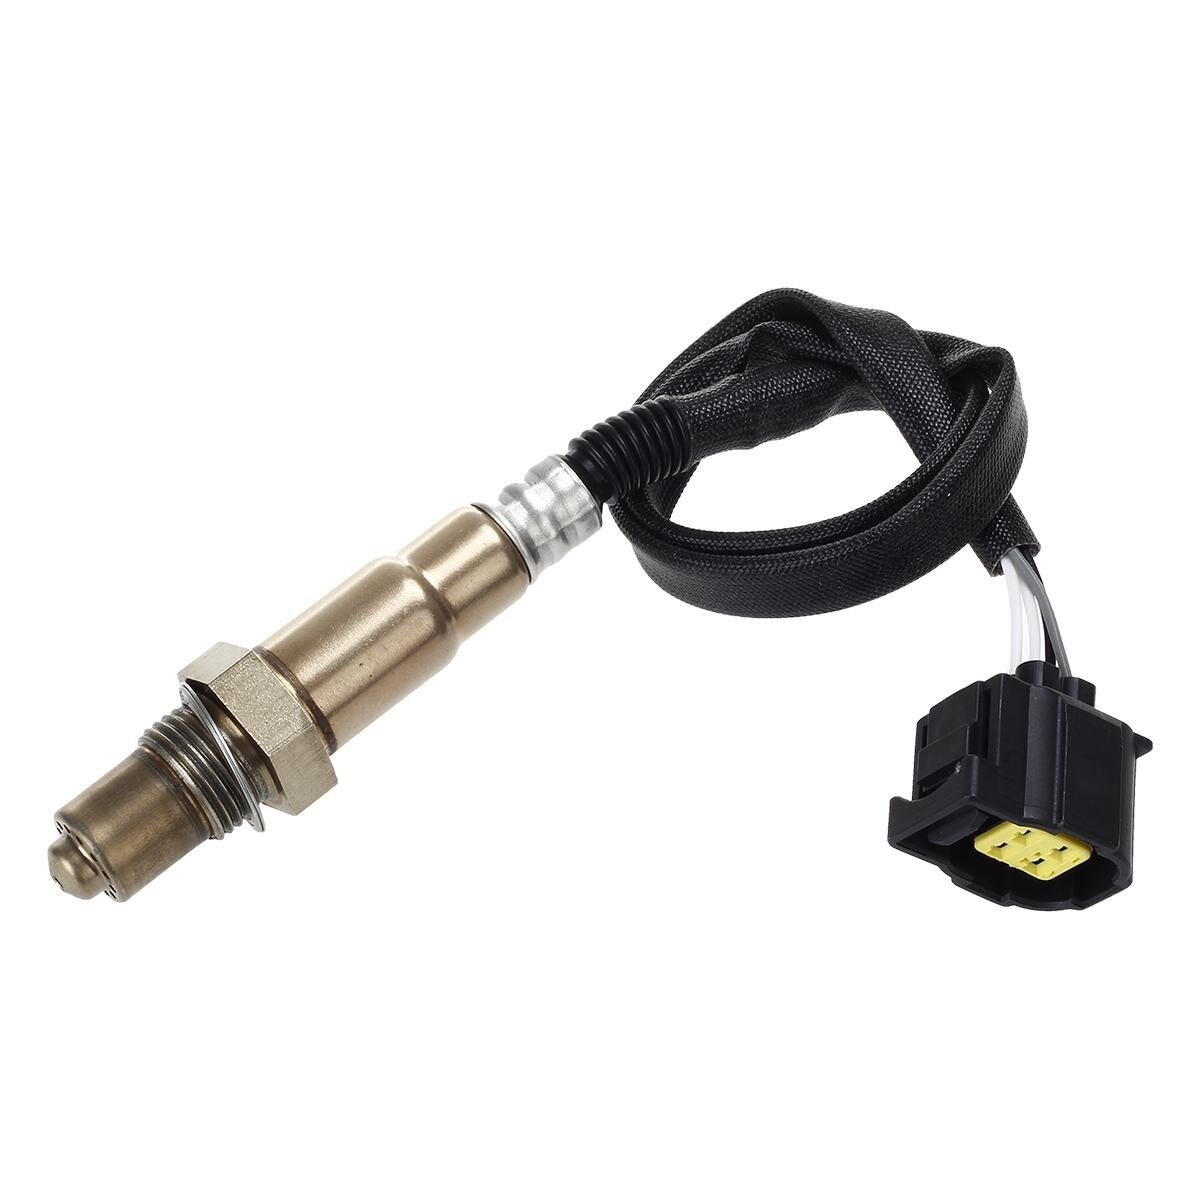
\includegraphics[width=0.5\textwidth]{Bilder/Oxygen_Sensor}
   \end{figure}


	
   \begin{minipage} [c] [3.5cm] [b] {\textwidth}
    \begin{center}
       Ausarbeitung als Beispiel\\
       \textcolor{green} {OBACHT! Bitte in Adobe\texttrademark Acrobat öffnen um Tipps zu sehen!}\\
       \url{https://acrobat.adobe.com/de/de/acrobat/pdf-reader.html}\\
       \vspace{0.3cm}
       Gruppe 00\\
       Torsten Reitmeier\\
       Klaus Falkner\\
       \vspace{0.5cm}
       \texttt{Dokument-Version: 02}\\
	\end{center}
  
   \end{minipage}


\end{titlepage}


\tableofcontents

\defineavatar{Newton}{color=lime,subject={Tip},icon=Check,author={T. Reitmeier}}
\pdfcommentsetup{avatar=Newton}

%%%%%%%%%%%%%%%%%%%%%%%%%%%%%%%%%%%%%%%%%%%%%%%%%%%%%%%%%%%%%%%%%%%%%

\chapter{Beschreibung des Versuchs}
\label{Grundlagen}
Mit Hilfe einer Sprungantwort der Zelle einer Lambdasonde \cite{TRMT} \pdfcomment{Verweis auf Quelle} soll deren Charakteristik bestimmt werden. Dazu dient der vorhandene Versuchsaufbau (siehe Abbildung \ref{gAufbau}), der die Sonde bereits auf die notwendige Temperatur von \SI{700}{\celsius} heizt.\\
Die digital einstellbare Stromquelle ($I_\mt{p}$) ist für den Versuchsteil a) so zu steuern, dass die vom AD-Wandler gemessene (und an den PC übertragene) Spannung $V_\mt{s}$ im Bereich $\SI{300}{mV} \pm \SI{50}{mV}$ \pdfcomment{1/2 Leerzeichen zw. Zahl und Einheit - SI-package} liegt.\\ 
Anschließend ist ein Sprung von $\SI{1}{\%}$ des unter a) benötigten Stroms additiv aufzuschalten und die Antwort des Systems für \SI{3}{s} aufzuzeichnen. Mithilfe dieser Sprungantwort erfolgt die Bestimmung der Übertragungsfunktion $G(s)=\cfrac{V_\mt{s}}{I_\mt{p}}$.

\begin{figure}[H]
 \begin{center}
 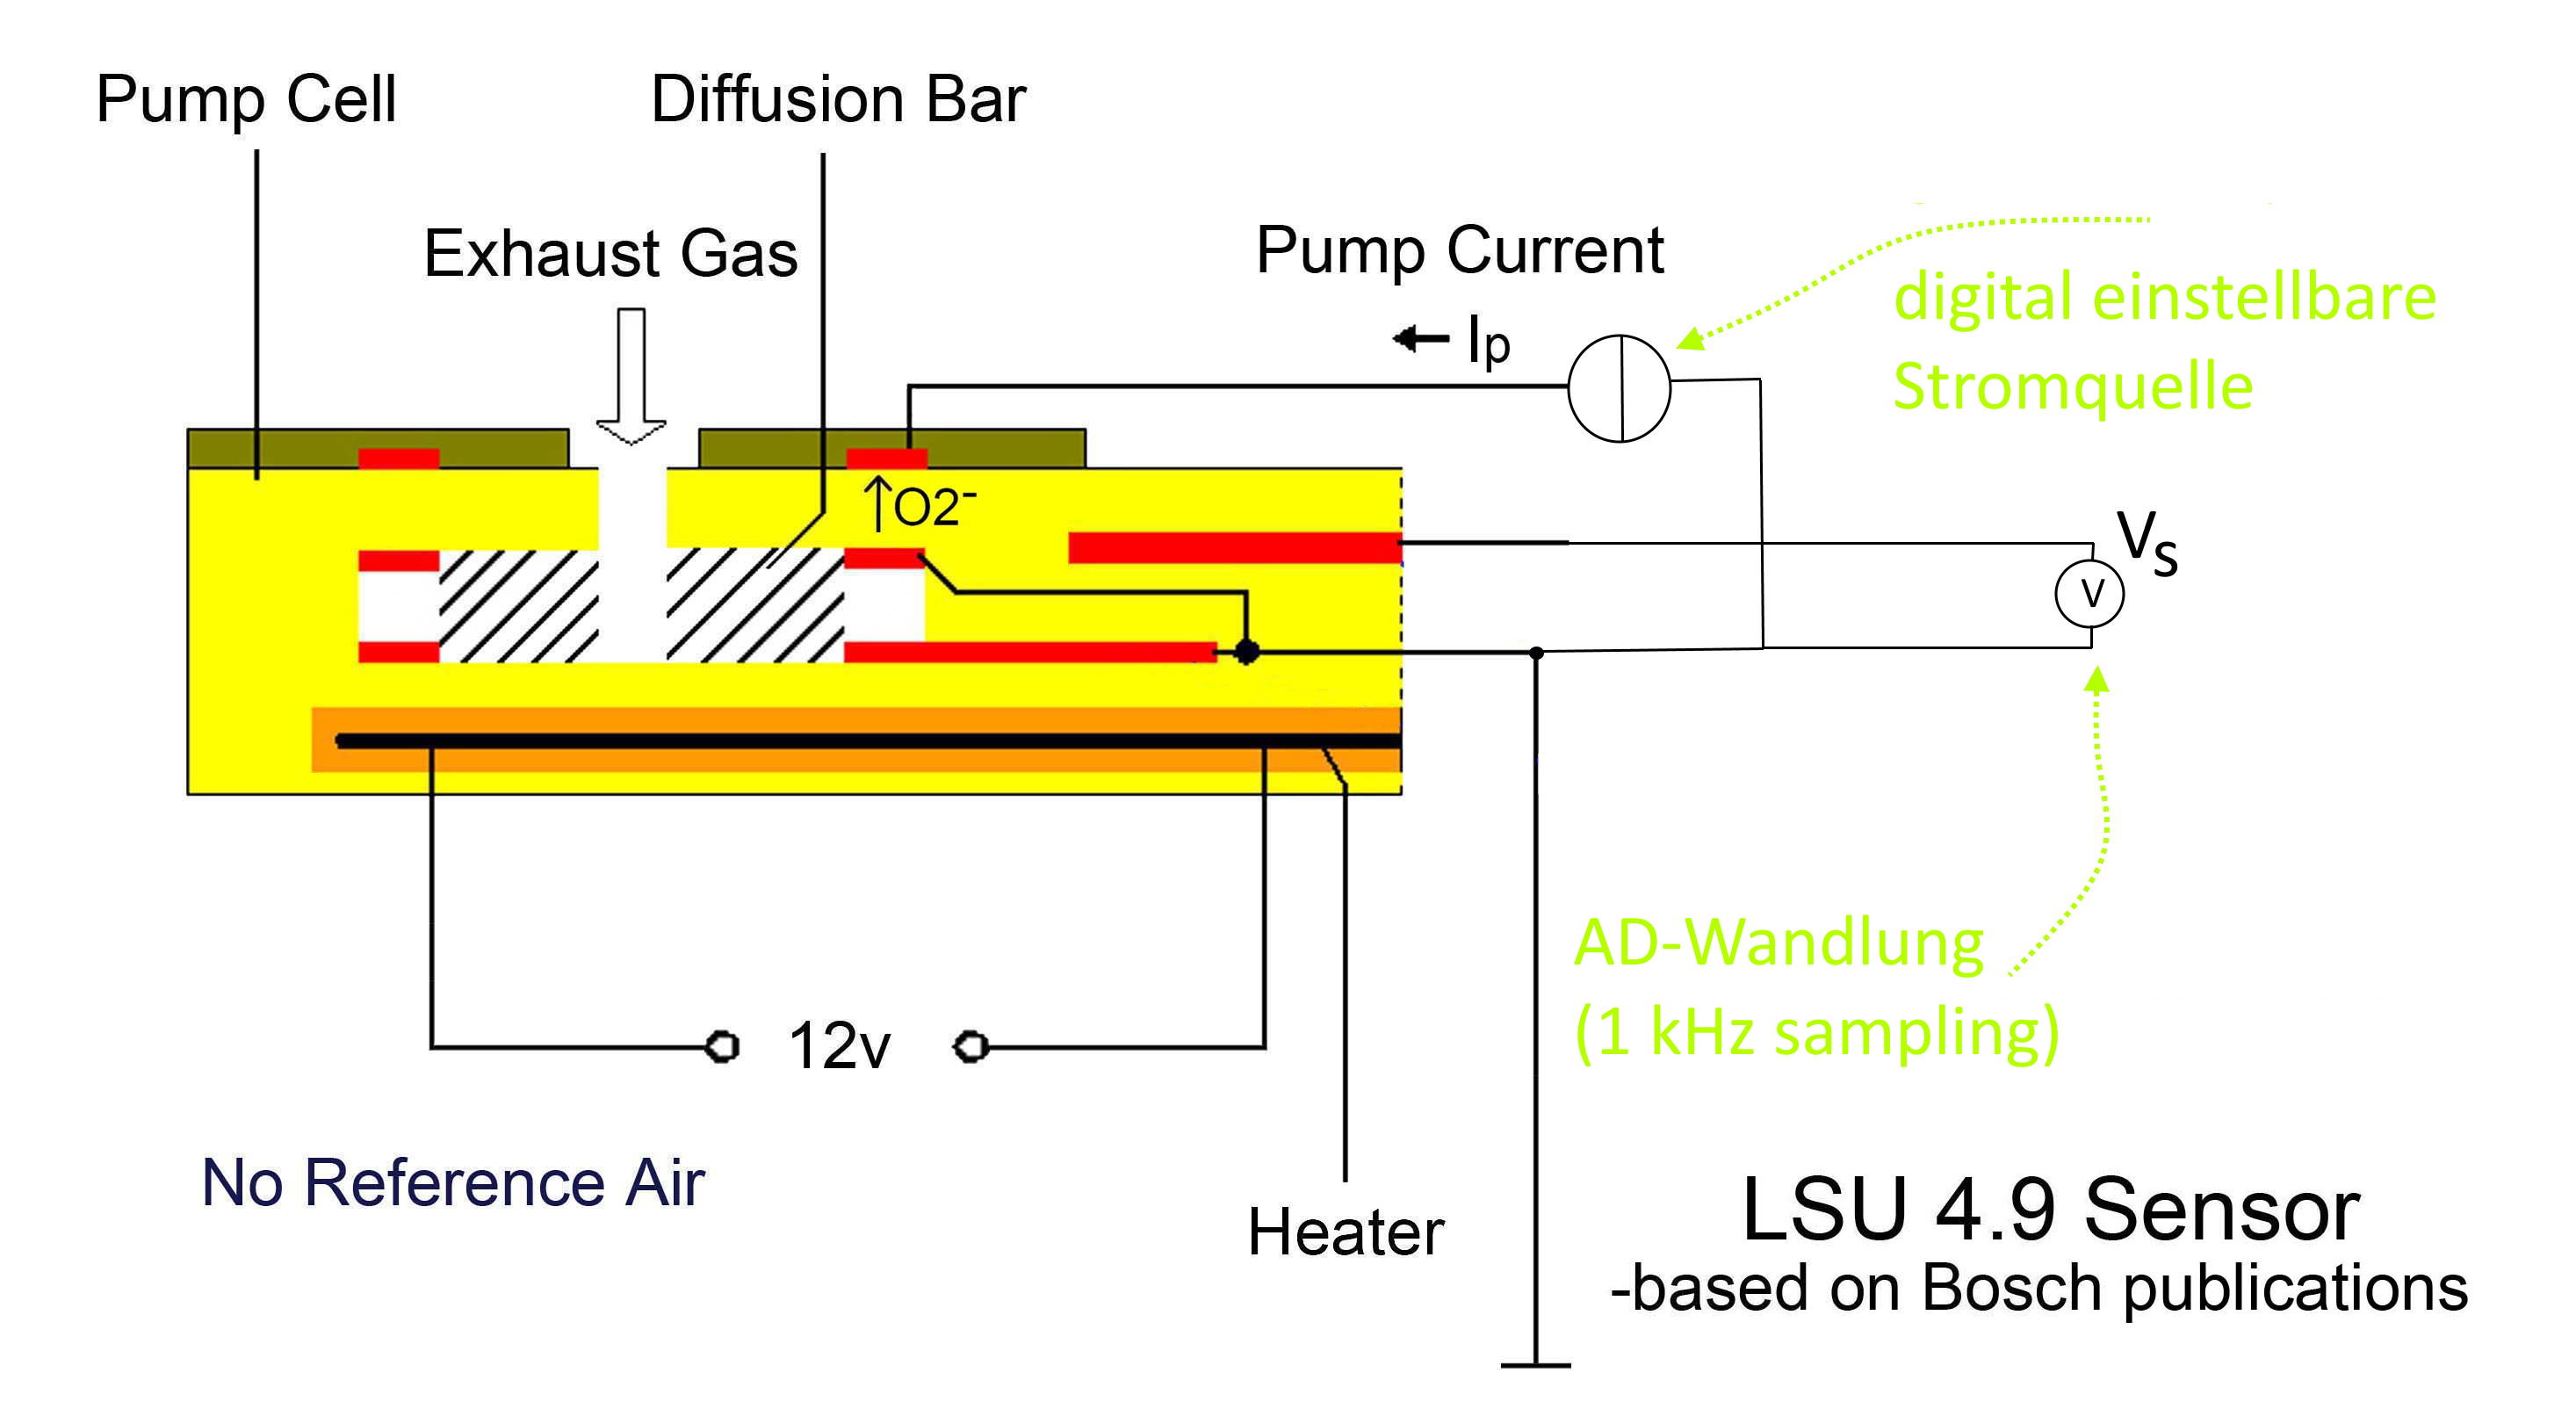
\includegraphics[width=1.0\textwidth]{./Bilder/LSU4.9}
 \end{center}
 \pdfcomment{BildUNTERschrift!, auf Abbildung ist im Text zu verweisen!}
 \caption{Skizze des Versuchsaufbaus}
 \label{gAufbau}
\end{figure}

%%%%%%%%%%%%%%%%%%%%%%%%%%%%%%%%%%%%%%%%%%%%%%%%%%%%%%%%%%%%%%%%%%%%%%

\chapter{Ergebnisse}
\label{erg}

\section{Daten stationärer Zustand}
\label{stat}
Der benötigte Strom für eine Spannung $V_\mt{s}=\SI{337}{mV}$ beträgt $I_\mt{p}=\SI{2.315}{mA}$.\\ 
Somit ist für die Höhe des Sprungs mit $\Delta I_\mt{p} \approx \SI{25}{uA}$ festzulegen.

\section{Sprungantwort $\frac{x_\mt{a}(t)}{x_\mt{e}(t)}=\frac{V_\mt{s}(t)}{I_\mt{p}(t)}$}
\label{ht}
Die Abbildung \ref{ght} zeigt die aufgezeichnete Sprungantwort - laut ermittelter Werte des stationären Zustands - im kompletten Aufzeichnungsbereich, während Abbildung \ref{ghtzoom} einen Ausschnitt kurz nach Aufschalten des Sprungs darstellt. Diese Darstellung ist zur Unterscheidung von $PT_1$ und $PT_\mt{n}$ ($n \geq 2$) notwendig \cite{TRRT, RSSCRIPT}.\\
\newline
Für $\mt{PT}_1$ gilt

\begin{equation}
 \frac{dV_\mt{s}(t=t_\mt{Sprung})}{dt} \neq 0 .
\end{equation}

Für $\mt{PT}_\mt{n}$ mit $n \geq 2$ gilt
\begin{equation}
 \frac{dV_\mt{s}(t=t_\mt{Sprung})}{dt} = 0 .
\end{equation}

\newpage

\begin{figure}[H]
 \begin{center}
 \hspace*{-0.2cm}
 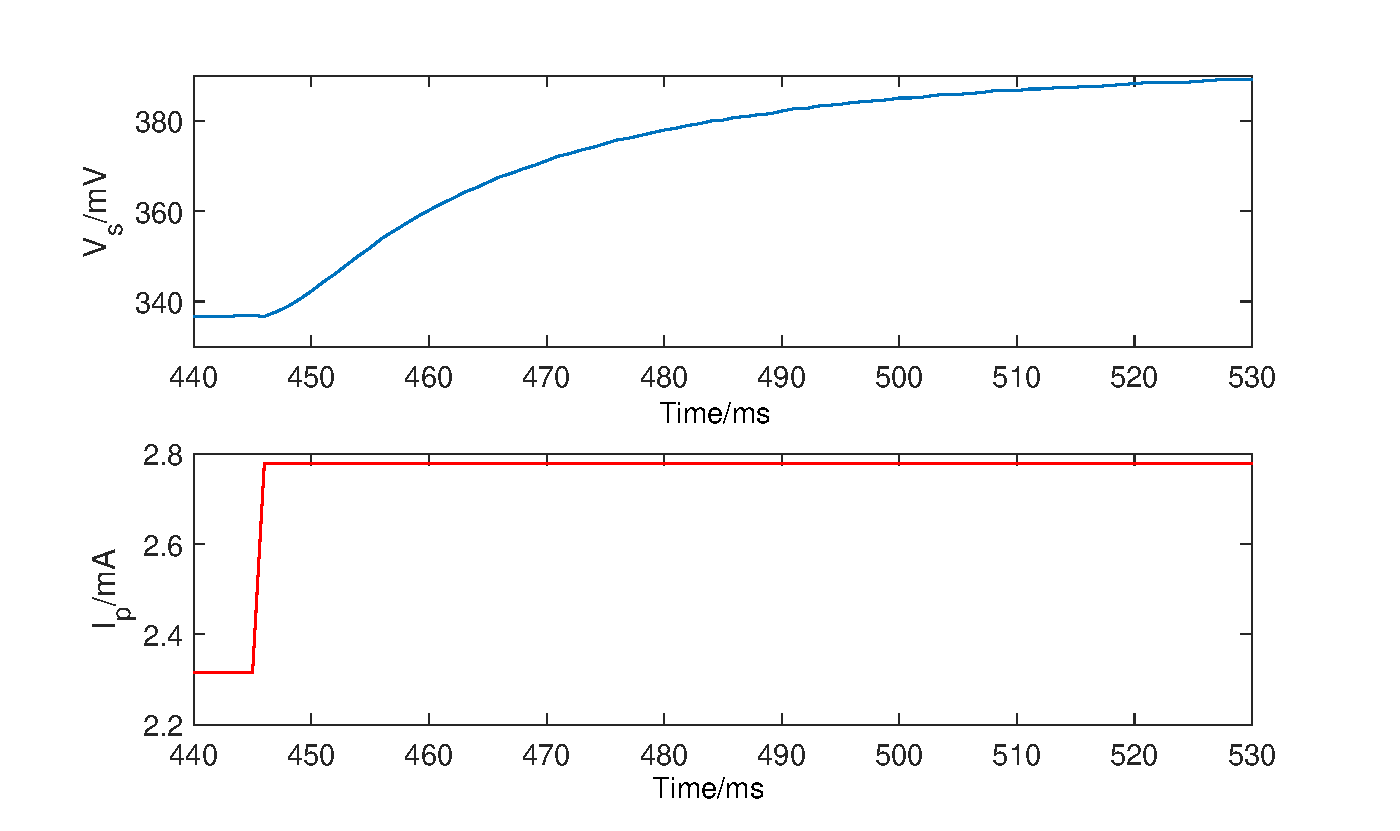
\includegraphics[width=0.95\textwidth]{./Bilder/h_t}
 \end{center}
 \vspace{-0.5cm}
 \caption{Sprungantwort  $I_\mt{p0}=\SI{2.315}{mA}$ $\longmapsto$ $I_\mt{p1}=\SI{2.778}{mA}$}
 \label{ght}
\end{figure}


\begin{figure}[H]
 \begin{center}
 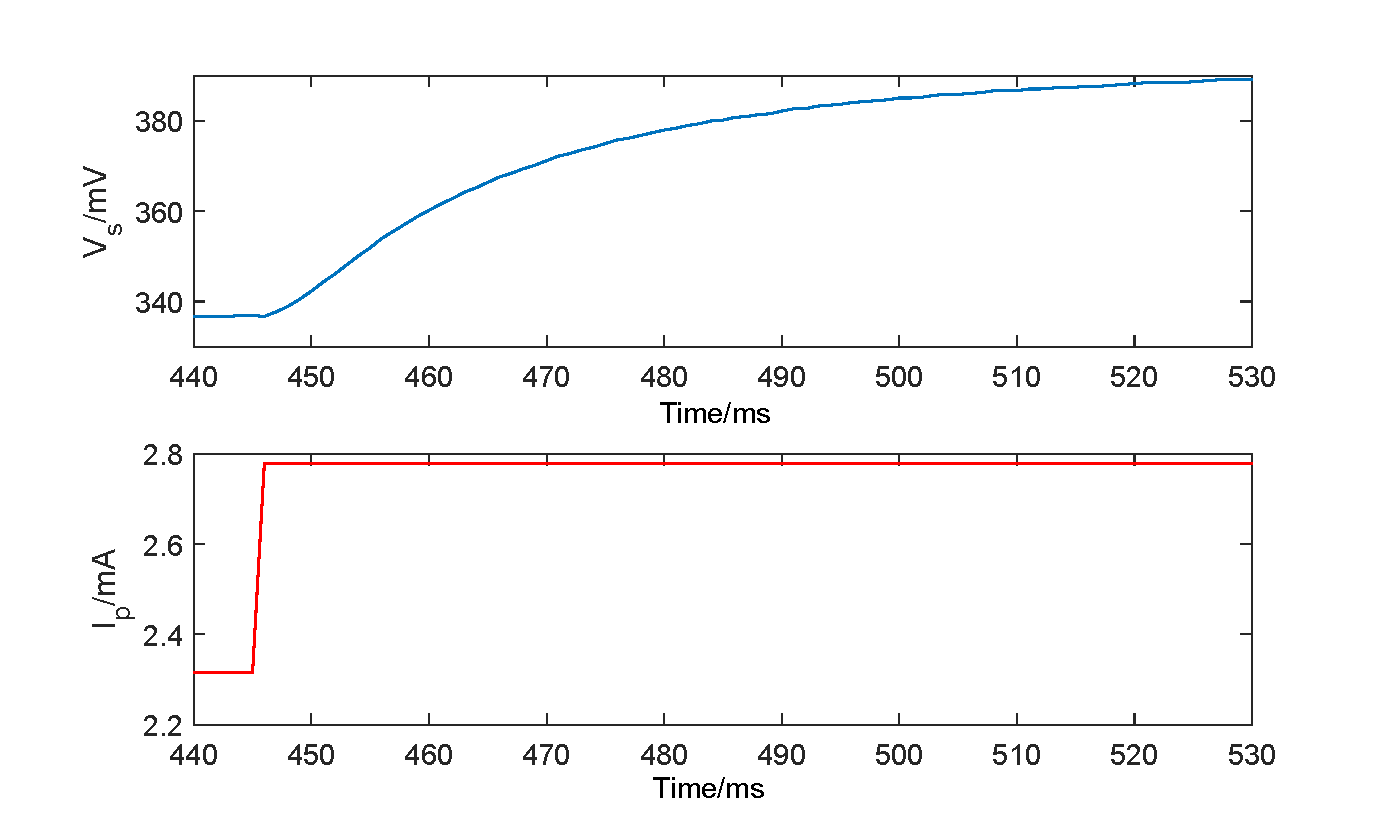
\includegraphics[width=0.95\textwidth]{./Bilder/h_t_zoom}
 \pdfcomment{Achsenbeschriftungen als zugeschnittene Größengleichungen, KEINESFALLS [] verwenden!}
 \end{center}
 \vspace{-0.5cm}
 \caption{Sprungantwort  $I_\mt{p0}=\SI{2.315}{mA}$ $\longmapsto$ $I_\mt{p1}=\SI{2.778}{mA}$ - Zoom}
 \label{ghtzoom}
\end{figure}

\newpage

%%%%%%%%%%%%%%%%%%%%%%%%%%%%%%%%%%%%%%%%%%%%%%%%%%%%%%%%%%%%%%%%%%%%%

\chapter{Auswertung}
\label{asw}

\section{Wahl des Modellansatzes}
\label{ModAnsatz}
Abbildung \ref{ghtzoom} zeigt $\cfrac{dV_\mt{s}}{dt} \rightarrow$ 0 zum Zeitpunkt des Sprungs. Es handelt sich somit um kein $PT_1$-Verhalten.\\
Mit Hilfe des Matlab\cite{MATLAB}-Tools \texttt{System Identification} wird nun versucht ein $PT_2$-System an die Messdaten anzupassen. 

\section{$\mt{PT}_2$-Modell}
\label{PT2}
Das Ergebnis der Anpassung zeigt die folgende Abbildung:\\
\vspace{-1cm}
\begin{figure}[H]
 \begin{center}
  \setlength\fwidth{0.85\textwidth}
  % This file was created by matlab2tikz.
%
%The latest updates can be retrieved from
%  http://www.mathworks.com/matlabcentral/fileexchange/22022-matlab2tikz-matlab2tikz
%where you can also make suggestions and rate matlab2tikz.
%
\definecolor{mycolor1}{rgb}{0.92941,0.69412,0.12549}%
%
\begin{tikzpicture}

\begin{axis}[%
width=0.951\fwidth,
height=0.613\fwidth,
at={(0\fwidth,0\fwidth)},
scale only axis,
xmin=0,
xmax=3,
xlabel style={font=\color{white!15!black}},
xlabel={Time/s},
ymin=330,
ymax=410,
ylabel style={font=\color{white!15!black}},
ylabel={Vs/mV},
axis background/.style={fill=white},
legend style={at={(0.724,0.704)}, anchor=south west, legend cell align=left, align=left, draw=white!15!black}
]
\addplot [color=mycolor1, dashdotted, line width=1.0pt]
  table[row sep=crcr]{%
0	336.940713216167\\
0.000999999999976353	336.373822050856\\
0.0199999999999818	365.467920751545\\
0.0289999999999964	373.280210688897\\
0.0380000000000109	378.704965344944\\
0.0480000000000018	382.828878409987\\
0.0579999999999927	385.608849429757\\
0.0679999999999836	387.500747499672\\
0.0779999999999745	388.805489224579\\
0.0880000000000223	389.721713459742\\
0.0989999999999895	390.43590423248\\
0.110000000000014	390.951093485911\\
0.122000000000014	391.369778043158\\
0.134999999999991	391.718810508388\\
0.15100000000001	392.060594381722\\
0.170000000000016	392.396876958472\\
0.194999999999993	392.780591642246\\
0.228000000000009	393.235955872766\\
0.267999999999972	393.743167264588\\
0.310999999999979	394.247805527317\\
0.353999999999985	394.715717676654\\
0.398000000000025	395.159690980571\\
0.442000000000007	395.571083437483\\
0.48599999999999	395.952297347582\\
0.529999999999973	396.305548347704\\
0.574000000000012	396.632887874775\\
0.617999999999995	396.936216620125\\
0.661999999999978	397.217295813534\\
0.706000000000017	397.477757489351\\
0.75	397.719113969003\\
0.793999999999983	397.94276664303\\
0.838000000000022	398.150014108161\\
0.882000000000005	398.342059707394\\
0.925999999999988	398.520018516981\\
0.970000000000027	398.684923820909\\
1.01400000000001	398.837733110467\\
1.05799999999999	398.979333643738\\
1.10300000000001	399.113415100997\\
1.14800000000002	399.237446580711\\
1.19299999999998	399.352181371595\\
1.238	399.458316300159\\
1.28300000000002	399.556495962792\\
1.32900000000001	399.649255597182\\
1.375	399.734914065205\\
1.42200000000003	399.815665581073\\
1.46899999999999	399.890106209287\\
1.517	399.960129407571\\
1.565	400.024568491852\\
1.61399999999998	400.08505254922\\
1.66399999999999	400.141702525763\\
1.71499999999997	400.194648504294\\
1.767	400.244028085174\\
1.82100000000003	400.290812056734\\
1.87599999999998	400.334172309796\\
1.93299999999999	400.374958027586\\
1.99200000000002	400.413142428172\\
2.053	400.448726946254\\
2.11599999999999	400.481738477291\\
2.18200000000002	400.51266924027\\
2.25099999999998	400.541440743795\\
2.32400000000001	400.568361061728\\
2.40100000000001	400.593300457463\\
2.483	400.616446344238\\
2.57100000000003	400.637889268164\\
2.666	400.657649539793\\
2.76799999999997	400.675542378871\\
2.88	400.691871271808\\
2.96300000000002	400.702085302223\\
};
\addlegendentry{Modellwerte}

\addplot [color=black, line width=1.0pt]
  table[row sep=crcr]{%
0	336.9\\
0.000999999999976353	336.7\\
0.0040000000000191	340.5\\
0.0190000000000055	365.2\\
0.0260000000000105	372.2\\
0.0419999999999732	381\\
0.0509999999999877	384.1\\
0.0690000000000168	387.5\\
0.0740000000000123	388.1\\
0.0769999999999982	388.5\\
0.0790000000000077	388.5\\
0.0840000000000032	389.3\\
0.0860000000000127	389.3\\
0.0880000000000223	389.5\\
0.089999999999975	389.5\\
0.0930000000000177	389.9\\
0.0960000000000036	390.1\\
0.0980000000000132	390.1\\
0.100000000000023	390.3\\
0.105000000000018	390.7\\
0.108000000000004	390.9\\
0.113	390.9\\
0.115000000000009	391.1\\
0.117000000000019	391.1\\
0.119000000000028	391.3\\
0.120999999999981	391.3\\
0.12299999999999	391.5\\
0.125	391.5\\
0.12700000000001	391.7\\
0.134000000000015	391.7\\
0.136000000000024	391.9\\
0.13900000000001	391.9\\
0.14100000000002	392.1\\
0.144999999999982	392.1\\
0.146999999999991	392.3\\
0.15100000000001	392.3\\
0.151999999999987	392.5\\
0.15300000000002	392.3\\
0.154999999999973	392.5\\
0.163000000000011	392.5\\
0.163999999999987	392.7\\
0.16500000000002	392.5\\
0.165999999999997	392.7\\
0.166999999999973	392.5\\
0.168999999999983	392.7\\
0.172000000000025	392.7\\
0.173000000000002	392.9\\
0.175000000000011	392.7\\
0.177000000000021	392.9\\
0.180000000000007	392.9\\
0.182000000000016	393.1\\
0.189999999999998	393.1\\
0.192000000000007	393.3\\
0.209000000000003	393.3\\
0.211000000000013	393.5\\
0.218999999999994	393.5\\
0.221000000000004	393.7\\
0.22199999999998	393.5\\
0.22399999999999	393.7\\
0.230999999999995	393.7\\
0.233000000000004	393.9\\
0.23399999999998	393.7\\
0.23599999999999	393.9\\
0.244000000000028	393.9\\
0.245999999999981	394.1\\
0.24799999999999	393.9\\
0.25	394.1\\
0.261000000000024	394.1\\
0.262	394.3\\
0.262999999999977	394.1\\
0.264999999999986	394.3\\
0.288000000000011	394.3\\
0.288999999999987	394.5\\
0.290999999999997	394.3\\
0.291999999999973	394.5\\
0.293000000000006	394.3\\
0.295000000000016	394.5\\
0.307000000000016	394.5\\
0.309000000000026	394.7\\
0.310999999999979	394.5\\
0.312999999999988	394.7\\
0.322999999999979	394.7\\
0.324999999999989	394.9\\
0.326999999999998	394.7\\
0.329000000000008	394.9\\
0.331000000000017	394.7\\
0.333000000000027	394.7\\
0.33499999999998	394.9\\
0.346000000000004	394.9\\
0.348000000000013	395.1\\
0.39100000000002	395.1\\
0.391999999999996	395.3\\
0.392999999999972	395.1\\
0.394999999999982	395.3\\
0.396999999999991	395.1\\
0.399000000000001	395.3\\
0.413000000000011	395.3\\
0.41500000000002	395.5\\
0.416999999999973	395.3\\
0.418999999999983	395.5\\
0.435000000000002	395.5\\
0.435999999999979	395.7\\
0.437999999999988	395.5\\
0.439999999999998	395.7\\
0.459000000000003	395.7\\
0.45999999999998	395.9\\
0.461999999999989	395.7\\
0.463999999999999	395.9\\
0.466999999999985	395.7\\
0.468999999999994	395.9\\
0.47399999999999	395.9\\
0.475000000000023	395.7\\
0.476999999999975	395.9\\
0.511000000000024	395.9\\
0.512999999999977	396.1\\
0.51400000000001	395.9\\
0.514999999999986	396.1\\
0.51600000000002	395.9\\
0.517999999999972	396.1\\
0.536999999999978	396.1\\
0.538999999999987	396.3\\
0.54000000000002	396.1\\
0.541999999999973	396.3\\
0.562999999999988	396.3\\
0.564000000000021	396.5\\
0.564999999999998	396.3\\
0.565999999999974	396.5\\
0.567999999999984	396.3\\
0.569000000000017	396.5\\
0.571000000000026	396.3\\
0.576000000000022	396.3\\
0.577999999999975	396.5\\
0.579999999999984	396.3\\
0.581999999999994	396.5\\
0.593999999999994	396.5\\
0.595000000000027	396.7\\
0.596000000000004	396.5\\
0.598000000000013	396.7\\
0.653999999999996	396.7\\
0.654999999999973	396.9\\
0.656999999999982	396.7\\
0.660000000000025	396.9\\
0.663000000000011	396.9\\
0.663999999999987	396.7\\
0.665999999999997	396.9\\
0.668000000000006	396.7\\
0.670000000000016	396.9\\
0.689999999999998	396.9\\
0.690999999999974	397.1\\
0.692999999999984	396.9\\
0.697000000000003	396.9\\
0.699000000000012	397.1\\
0.699999999999989	396.9\\
0.701999999999998	397.1\\
0.706999999999994	397.1\\
0.708000000000027	397.3\\
0.70999999999998	397.1\\
0.711000000000013	397.3\\
0.713000000000022	397.1\\
0.713999999999999	397.3\\
0.716000000000008	397.1\\
0.721000000000004	397.1\\
0.72199999999998	397.3\\
0.72399999999999	397.1\\
0.726999999999975	397.3\\
0.75	397.3\\
0.750999999999976	397.5\\
0.75200000000001	397.3\\
0.752999999999986	397.5\\
0.754000000000019	397.3\\
0.755999999999972	397.5\\
0.757000000000005	397.3\\
0.759000000000015	397.5\\
0.824000000000012	397.5\\
0.824999999999989	397.7\\
0.826999999999998	397.5\\
0.834000000000003	397.5\\
0.83499999999998	397.7\\
0.836999999999989	397.5\\
0.838999999999999	397.7\\
0.839999999999975	397.5\\
0.841999999999985	397.7\\
0.853000000000009	397.7\\
0.853999999999985	397.9\\
0.855999999999995	397.7\\
0.858000000000004	397.7\\
0.85899999999998	397.9\\
0.86099999999999	397.7\\
0.862000000000023	397.9\\
0.863	397.7\\
0.865000000000009	397.9\\
0.865999999999985	397.7\\
0.867999999999995	397.9\\
0.869000000000028	397.7\\
0.870000000000005	397.9\\
0.870999999999981	397.7\\
0.87299999999999	397.9\\
0.879000000000019	397.9\\
0.879999999999995	397.7\\
0.882000000000005	397.9\\
0.904999999999973	397.9\\
0.906000000000006	398.1\\
0.908000000000015	397.9\\
0.910000000000025	397.9\\
0.911999999999978	398.1\\
0.951999999999998	398.1\\
0.952999999999975	398.3\\
0.954999999999984	398.1\\
0.958000000000027	398.1\\
0.95999999999998	398.3\\
1.02600000000001	398.3\\
1.02699999999999	398.5\\
1.029	398.3\\
1.02999999999997	398.5\\
1.03100000000001	398.3\\
1.03199999999998	398.5\\
1.03399999999999	398.3\\
1.03699999999998	398.3\\
1.03899999999999	398.5\\
1.07799999999997	398.5\\
1.07900000000001	398.7\\
1.07999999999998	398.5\\
1.08199999999999	398.7\\
1.08800000000002	398.7\\
1.089	398.5\\
1.08999999999997	398.7\\
1.09100000000001	398.5\\
1.09300000000002	398.7\\
1.12	398.7\\
1.12099999999998	398.9\\
1.12299999999999	398.7\\
1.12599999999998	398.7\\
1.12799999999999	398.9\\
1.13	398.7\\
1.13099999999997	398.9\\
1.13200000000001	398.7\\
1.13400000000001	398.9\\
1.13600000000002	398.7\\
1.13900000000001	398.9\\
1.17500000000001	398.9\\
1.17599999999999	399.1\\
1.178	398.9\\
1.18599999999998	398.9\\
1.18700000000001	399.1\\
1.18900000000002	398.9\\
1.19	399.1\\
1.19200000000001	398.9\\
1.19600000000003	398.9\\
1.197	399.1\\
1.19799999999998	398.9\\
1.19999999999999	399.1\\
1.20100000000002	398.9\\
1.20299999999997	399.1\\
1.20499999999998	399.1\\
1.20600000000002	398.9\\
1.20800000000003	399.1\\
1.27800000000002	399.1\\
1.279	399.3\\
1.28100000000001	399.1\\
1.29199999999997	399.1\\
1.29399999999998	399.3\\
1.29599999999999	399.3\\
1.298	399.1\\
1.30099999999999	399.3\\
1.34300000000002	399.3\\
1.34399999999999	399.5\\
1.34500000000003	399.3\\
1.346	399.5\\
1.34699999999998	399.3\\
1.34800000000001	399.5\\
1.35000000000002	399.3\\
1.35399999999998	399.3\\
1.35500000000002	399.5\\
1.35700000000003	399.3\\
1.36000000000001	399.5\\
1.36700000000002	399.5\\
1.36799999999999	399.3\\
1.37	399.5\\
1.375	399.5\\
1.37599999999998	399.3\\
1.37799999999999	399.5\\
1.42000000000002	399.5\\
1.42099999999999	399.7\\
1.423	399.5\\
1.42500000000001	399.7\\
1.42700000000002	399.5\\
1.42899999999997	399.7\\
1.43099999999998	399.7\\
1.43299999999999	399.5\\
1.435	399.7\\
1.44799999999998	399.7\\
1.44900000000001	399.5\\
1.45100000000002	399.7\\
1.45999999999998	399.7\\
1.46100000000001	399.9\\
1.46300000000002	399.7\\
1.47399999999999	399.7\\
1.47500000000002	399.9\\
1.47699999999998	399.7\\
1.47800000000001	399.9\\
1.47899999999998	399.7\\
1.48099999999999	399.9\\
1.483	399.7\\
1.48500000000001	399.9\\
1.488	399.9\\
1.48899999999998	399.7\\
1.49099999999999	399.9\\
1.49400000000003	399.9\\
1.495	399.7\\
1.49599999999998	399.9\\
1.49700000000001	399.7\\
1.49900000000002	399.9\\
1.54300000000001	399.9\\
1.54399999999998	400.1\\
1.54599999999999	399.9\\
1.56200000000001	399.9\\
1.56299999999999	400.1\\
1.56400000000002	399.9\\
1.565	400.1\\
1.56700000000001	399.9\\
1.57100000000003	399.9\\
1.57299999999998	400.1\\
1.57499999999999	399.9\\
1.577	400.1\\
1.57799999999997	399.9\\
1.57999999999998	400.1\\
1.58100000000002	399.9\\
1.58300000000003	400.1\\
1.58499999999998	400.1\\
1.58699999999999	399.9\\
1.58800000000002	400.1\\
1.589	399.9\\
1.59100000000001	400.1\\
1.59199999999998	399.9\\
1.59399999999999	400.1\\
1.59500000000003	399.9\\
1.59699999999998	400.1\\
1.81700000000001	400.1\\
1.81799999999998	400.3\\
1.81999999999999	400.1\\
1.82299999999998	400.3\\
1.82499999999999	400.1\\
1.827	400.1\\
1.82799999999997	400.3\\
1.82999999999998	400.1\\
1.83199999999999	400.3\\
1.834	400.1\\
1.83699999999999	400.3\\
1.839	400.1\\
1.84100000000001	400.3\\
1.84300000000002	400.1\\
1.84500000000003	400.3\\
1.846	400.1\\
1.84800000000001	400.3\\
1.85000000000002	400.3\\
1.851	400.1\\
1.85300000000001	400.3\\
1.875	400.3\\
1.87599999999998	400.1\\
1.87799999999999	400.3\\
1.88400000000001	400.3\\
1.88499999999999	400.1\\
1.88600000000002	400.3\\
1.887	400.1\\
1.88900000000001	400.3\\
1.89400000000001	400.3\\
1.89499999999998	400.1\\
1.89699999999999	400.3\\
1.90199999999999	400.3\\
1.90300000000002	400.1\\
1.90499999999997	400.3\\
1.93099999999998	400.3\\
1.93200000000002	400.1\\
1.93400000000003	400.3\\
1.95400000000001	400.3\\
1.95499999999998	400.1\\
1.95699999999999	400.3\\
1.983	400.3\\
1.98399999999998	400.5\\
1.98599999999999	400.3\\
2.01400000000001	400.3\\
2.01499999999999	400.5\\
2.017	400.3\\
2.02800000000002	400.3\\
2.029	400.5\\
2.03100000000001	400.3\\
2.03800000000001	400.3\\
2.04000000000002	400.5\\
2.04300000000001	400.3\\
2.05500000000001	400.3\\
2.05599999999998	400.5\\
2.05700000000002	400.3\\
2.05900000000003	400.5\\
2.06099999999998	400.3\\
2.06299999999999	400.5\\
2.065	400.3\\
2.06700000000001	400.3\\
2.06799999999998	400.5\\
2.06999999999999	400.3\\
2.07299999999998	400.3\\
2.07400000000001	400.5\\
2.07600000000002	400.3\\
2.077	400.5\\
2.07799999999997	400.3\\
2.07900000000001	400.5\\
2.07999999999998	400.3\\
2.08100000000002	400.5\\
2.08300000000003	400.3\\
2.084	400.5\\
2.08499999999998	400.3\\
2.08699999999999	400.5\\
2.089	400.5\\
2.09100000000001	400.3\\
2.09300000000002	400.5\\
2.09500000000003	400.3\\
2.09699999999998	400.5\\
2.10199999999998	400.5\\
2.10300000000001	400.3\\
2.10500000000002	400.5\\
2.108	400.5\\
2.11000000000001	400.3\\
2.11399999999998	400.3\\
2.11599999999999	400.5\\
2.11799999999999	400.3\\
2.12	400.3\\
2.12099999999998	400.5\\
2.12200000000001	400.3\\
2.12400000000002	400.5\\
2.12700000000001	400.3\\
2.12799999999999	400.5\\
2.12900000000002	400.3\\
2.13	400.5\\
2.13100000000003	400.3\\
2.13299999999998	400.5\\
2.13600000000002	400.3\\
2.13799999999998	400.5\\
2.142	400.5\\
2.14400000000001	400.3\\
2.14600000000002	400.5\\
2.15699999999998	400.5\\
2.15800000000002	400.3\\
2.16000000000003	400.5\\
2.25999999999999	400.5\\
2.26100000000002	400.7\\
2.262	400.5\\
2.26299999999998	400.7\\
2.26400000000001	400.5\\
2.26499999999999	400.7\\
2.267	400.5\\
2.27600000000001	400.5\\
2.27699999999999	400.7\\
2.279	400.5\\
2.27999999999997	400.7\\
2.28199999999998	400.5\\
2.28800000000001	400.5\\
2.28899999999999	400.7\\
2.291	400.5\\
2.29399999999998	400.5\\
2.29500000000002	400.7\\
2.29700000000003	400.5\\
2.30799999999999	400.5\\
2.30900000000003	400.7\\
2.31099999999998	400.5\\
2.31900000000002	400.5\\
2.31999999999999	400.7\\
2.322	400.5\\
2.32299999999998	400.7\\
2.32499999999999	400.5\\
2.34500000000003	400.5\\
2.346	400.7\\
2.34699999999998	400.5\\
2.34800000000001	400.7\\
2.34899999999999	400.5\\
2.35000000000002	400.7\\
2.35199999999998	400.5\\
2.35500000000002	400.7\\
2.35700000000003	400.5\\
2.35899999999998	400.5\\
2.36000000000001	400.7\\
2.36099999999999	400.5\\
2.363	400.7\\
2.36599999999999	400.5\\
2.36700000000002	400.7\\
2.36799999999999	400.5\\
2.36900000000003	400.7\\
2.37	400.5\\
2.37200000000001	400.7\\
2.375	400.5\\
2.37700000000001	400.7\\
2.38400000000001	400.7\\
2.38600000000002	400.5\\
2.38799999999998	400.5\\
2.38999999999999	400.7\\
2.392	400.5\\
2.39400000000001	400.7\\
2.40499999999997	400.7\\
2.40600000000001	400.5\\
2.40800000000002	400.7\\
2.41000000000003	400.5\\
2.411	400.7\\
2.41199999999998	400.5\\
2.41399999999999	400.7\\
2.488	400.7\\
2.48899999999998	400.9\\
2.49099999999999	400.7\\
2.49599999999998	400.7\\
2.49700000000001	400.9\\
2.49900000000002	400.7\\
2.52199999999999	400.7\\
2.52300000000002	400.9\\
2.52499999999998	400.7\\
2.53399999999999	400.7\\
2.53500000000003	400.9\\
2.53699999999998	400.7\\
2.54300000000001	400.7\\
2.54500000000002	400.9\\
2.54700000000003	400.7\\
2.565	400.7\\
2.56599999999997	400.9\\
2.56799999999998	400.7\\
2.57600000000002	400.7\\
2.57799999999997	400.9\\
2.57999999999998	400.7\\
2.58300000000003	400.7\\
2.58499999999998	400.9\\
2.58699999999999	400.7\\
2.589	400.7\\
2.59100000000001	400.9\\
2.59199999999998	400.7\\
2.59300000000002	400.9\\
2.59399999999999	400.7\\
2.59500000000003	400.9\\
2.596	400.7\\
2.59699999999998	400.9\\
2.59899999999999	400.7\\
2.601	400.9\\
2.60300000000001	400.7\\
2.60399999999998	400.9\\
2.60500000000002	400.7\\
2.60599999999999	400.9\\
2.608	400.7\\
2.61000000000001	400.9\\
2.61200000000002	400.7\\
2.61399999999998	400.9\\
2.61599999999999	400.7\\
2.61799999999999	400.9\\
2.62200000000001	400.9\\
2.62299999999999	400.7\\
2.62400000000002	400.9\\
2.625	400.7\\
2.62700000000001	400.9\\
2.62900000000002	400.7\\
2.63100000000003	400.9\\
2.63299999999998	400.7\\
2.63400000000001	400.9\\
2.63600000000002	400.7\\
2.63900000000001	400.7\\
2.63999999999999	400.9\\
2.642	400.7\\
2.64400000000001	400.9\\
2.64600000000002	400.7\\
2.649	400.9\\
2.65199999999999	400.7\\
2.65300000000002	400.9\\
2.654	400.7\\
2.65600000000001	400.9\\
2.65699999999998	400.7\\
2.65899999999999	400.9\\
2.661	400.7\\
2.66300000000001	400.9\\
2.66800000000001	400.9\\
2.66899999999998	400.7\\
2.67099999999999	400.9\\
2.67200000000003	400.7\\
2.673	400.9\\
2.67500000000001	400.7\\
2.67700000000002	400.9\\
2.67899999999997	400.7\\
2.68099999999998	400.9\\
2.68299999999999	400.7\\
2.68599999999998	400.7\\
2.68700000000001	400.9\\
2.68900000000002	400.7\\
2.69999999999999	400.7\\
2.702	400.9\\
2.70400000000001	400.7\\
2.709	400.7\\
2.70999999999998	400.9\\
2.71199999999999	400.7\\
2.71300000000002	400.9\\
2.71499999999997	400.7\\
2.72699999999998	400.7\\
2.72800000000001	400.9\\
2.73000000000002	400.7\\
2.73200000000003	400.9\\
2.73399999999998	400.7\\
2.786	400.7\\
2.78699999999998	400.9\\
2.78899999999999	400.7\\
2.84699999999998	400.7\\
2.84800000000001	400.5\\
2.85000000000002	400.7\\
2.86700000000002	400.7\\
2.86799999999999	400.5\\
2.87	400.7\\
2.875	400.7\\
2.87599999999998	400.5\\
2.87799999999999	400.7\\
2.88600000000002	400.7\\
2.887	400.5\\
2.88900000000001	400.7\\
2.89100000000002	400.7\\
2.89299999999997	400.5\\
2.89499999999998	400.7\\
2.89699999999999	400.7\\
2.89800000000002	400.5\\
2.899	400.7\\
2.89999999999998	400.5\\
2.90100000000001	400.7\\
2.90300000000002	400.5\\
2.90600000000001	400.7\\
2.90800000000002	400.5\\
2.91300000000001	400.5\\
2.91399999999999	400.7\\
2.916	400.5\\
2.91800000000001	400.7\\
2.92000000000002	400.5\\
2.92200000000003	400.7\\
2.923	400.5\\
2.92399999999998	400.7\\
2.92599999999999	400.5\\
2.92899999999997	400.5\\
2.93099999999998	400.7\\
2.93299999999999	400.5\\
2.93799999999999	400.5\\
2.93900000000002	400.7\\
2.94099999999997	400.5\\
2.96300000000002	400.5\\
};
\addlegendentry{Messdaten}

\end{axis}

\begin{axis}[%
width=1.227\fwidth,
height=0.752\fwidth,
at={(-0.16\fwidth,-0.083\fwidth)},
scale only axis,
xmin=0,
xmax=1,
ymin=0,
ymax=1,
axis line style={draw=none},
ticks=none,
axis x line*=bottom,
axis y line*=left
]
\end{axis}
\end{tikzpicture}%
  \pdfcomment{Kommando in Matlab: matlab2tikz('MessPT2.tex','width', '\fwidth' );}
  \pdfcomment{Reduzieren der Punkte auf z.B. 200: cleanfigure('targetResolution',200);}
 \end{center}
 \vspace{-1.0cm}
 \caption{Anpassung PT\textsubscript{2}-Glied}
 \label{gPT2}
\end{figure}

Es ist zu erkennen, dass der $\mt{PT}_2$-Ansatz mit den real gemessenen Daten gut korreliert.

Die Übertragungsfunktion sowie deren Parameter lauten

\begin{equation}
  G(s) = \frac{V_\mt{s}(s)}{I_\mt{p}(s)} = \frac{K_\mt{P}}{(1+s \cdot T_1) \cdot (1+s \cdot T_2)} .
\end{equation}

\begin{center}
 \captionof{table}{Parameter - Werte} \pdfcomment{Tabellen haben ÜBERschriften}
 \begin{tabular}{|p{2cm}|p{3cm}|}
 \hline
 Parameter & Wert   \\ \hline\hline
 $K_\mt{p}$ & $\SI{3201}{\cfrac{mV}{mA}}$    \\ \hline
 $T_1$ & \SI{0.7}{s}  \\ \hline
 $T_2$ & \SI{25}{ms}  \\ \hline
 \end{tabular}
\end{center}

\vspace{0.5cm}
Im Folgenden wird die Güte der Anpassung genauer untersucht.\\
\vspace{1cm}

\section{Überprüfung der Abweichung des Modells von den gemessenen Daten}
\label{check}
Um die Abweichung deutlich erkennen zu können, wurde die Differenz zwischen realen Daten und Modelldaten gebildet. Sie ist in folgender Abbildung dargestellt:\\

\begin{figure}[H]
 \begin{center}
 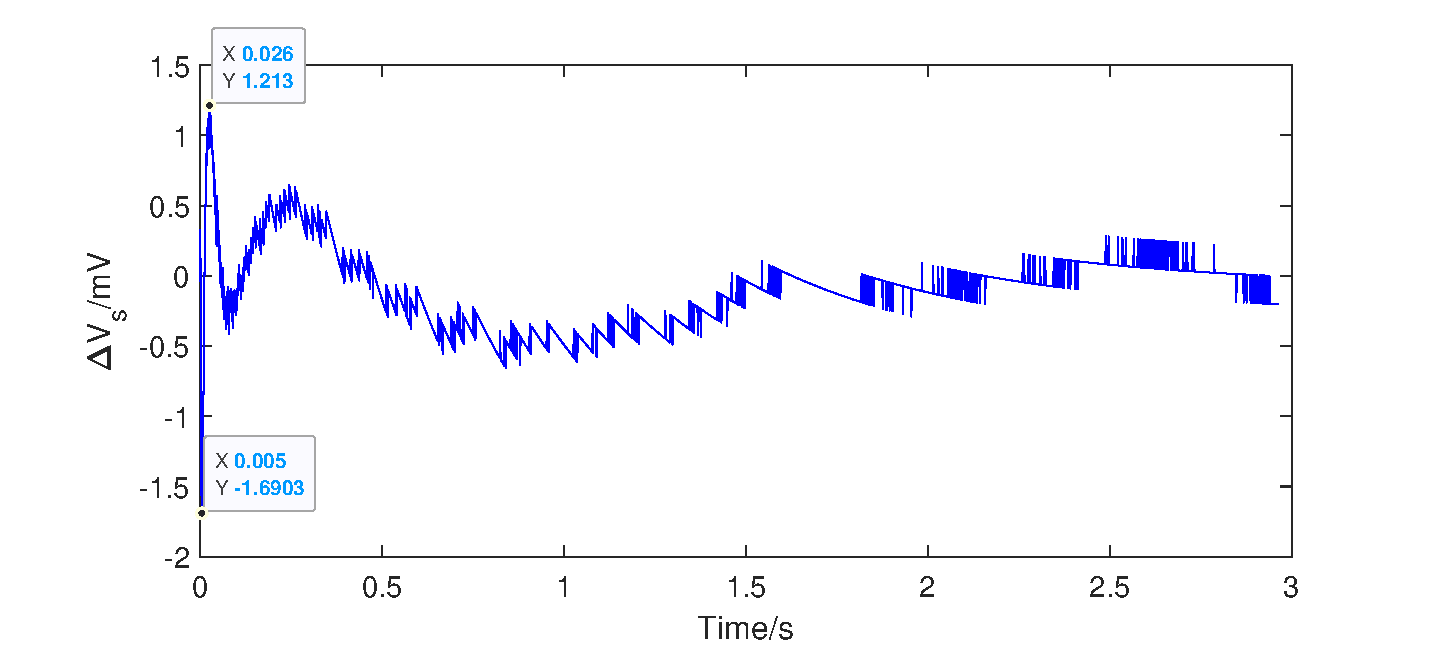
\includegraphics[width=0.9\textwidth]{./Bilder/Diff_Mess_PT2}
 \end{center}
 \vspace{-0.5cm}
 \caption{Differenz Messwerte zu Werten aus PT2-Modell}
 \label{gPT2Diff}
\end{figure}

%%%%%%%%%%%%%%%%%%%%%%%%%%%%%%%%%%%%%%%%%%%%%%%%%%%%%%%%%%%%%%%%%%%%%

\chapter{Fazit/Vorbereitung PI-Regler}

\section{Fazit}
\label{faz}
Laut Graphik \ref{gPT2Diff} liegt die Abweichung von Modell- zu realen Daten im Bereich $\pm 2mV$. Dies ist für die Modellbildung hinreichend genau. Es kann auf Basis dieses Modells im nächsten Versuch die Auslegung des PI-Reglers erfolgen. Ein I-Anteil im Regler ist zwingend erforderlich, damit der geschlossene Kreis bei einem $PT_2$-Streckenverhalten keine bleibende Regelabweichung besitzt \cite{TRRT}.\\


\section{Simulink-Modell mit PI-Regler}
In Vorbereitung auf den nächsten Versuch ist unten das Simulink-Modell mit Strecke und PI-Regler dargestellt.

\begin{figure}[H]
 \begin{center}
 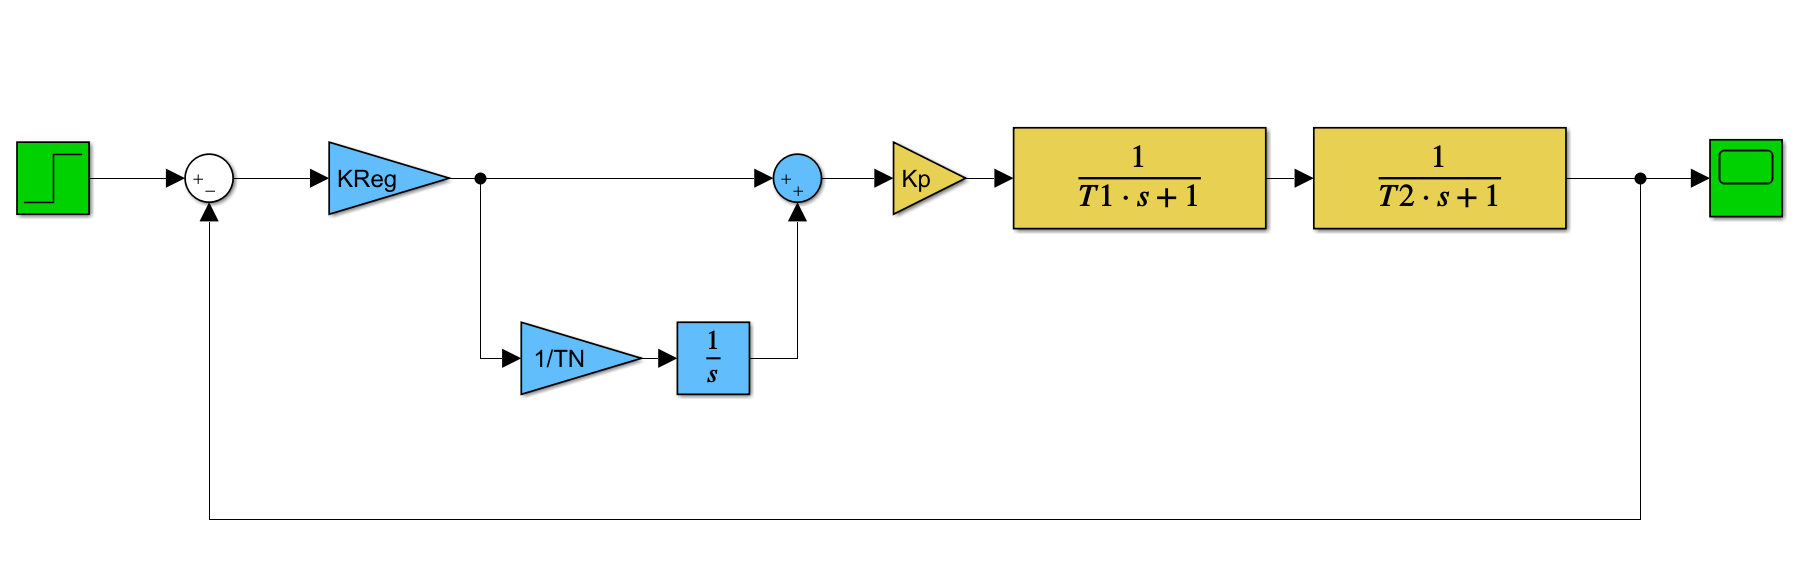
\includegraphics[width=1.0\textwidth]{./Bilder/Simulink}
 \pdfcomment{Screenshot in ausreichender Auflösung, Übertragungsfunktionen müssen lesbar sein - Boxgröße anpassen!}
 \end{center}
 \vspace{-0.5cm}
 \caption{Simulink-Ansatz $PT_2$-Strecke mit PI-Regler}
 \label{gSimMod}
\end{figure}

%%%%%%%%%%%%%%%%%%%%%%%%%%%%%%%%%%%%%%%%%%%%%%%%%%%%%%%%%%%%%%%%%%%%%

%%Addional hints
\chapter{Hinweise zu Grafiken}

Das Einbinden der Grafiken als \texttt{*.png} erfordert eine entsprechend hohe Auflösung um die berühmte \glqq verpixelte Grafik\grqq{} zu vermeiden. Dies wird leider häufig nicht beachtet, so dass Skalen, Beschriftungen, usw. unleserlich erscheinen.\\
\newline
Im Folgenden werden daher zwei Möglichkeiten zur Einbindung von Grafiken kurz beschrieben:

\begin{itemize}

\item Graphik als \texttt{*.eps} - Standard-Methode:\\
Matlab bietet die Möglichkeit die erzeugte Grafik als \textbf{e}ncapsulated \textbf{p}ost\textbf{s}cript zu speichern. Dies ist ein Vektorformat und kann verlustfrei in beliebigen Größen dargestellt werden.\\

\fbox{\begin{tabular}{@{}c@{}}
  \textbf{Obacht!} - Hintergrund des Diagramms: weiß, Beschriftung: schwarz!\\
  Kennlinien in deutlich sichtbaren, sich unterscheidenden Farben darstellen\\ 
  (z.B. gelb vermeiden)!
  \end{tabular}}

\vspace*{0.5cm}
Beispiele: Abbildungen \ref{ght}, \ref{ghtzoom}, \ref{gPT2Diff}
\vspace*{0.5cm}

\item Graphik mithilfe von \texttt{tikz} in LaTeX einbinden - für Technik-Freaks:\\
Per Skript wird aus dem Matlab/Octave-Graphen eine \texttt{*.tex}-Datei erzeugt, die den Graphen als \texttt{tikzpicture} darstellt. Dies hat den Vorteil, dass Attribute wie Schriftarten, Textgröße, ... des Dokuments verwendet werden. Ebenso sind Hintergrund, Farbgebung, ... automatisch definiert!\\
Quelle und Anleitung: \url{https://github.com/matlab2tikz/matlab2tikz}\\
\newline
Beachten Sie die Hinweise beim Graphen!

\vspace*{0.5cm}
Beispiel: Abbildung \ref{gPT2}
\vspace*{0.5cm}

\item Bei Verwendung von Word\textsuperscript{\texttrademark{}}  \texttt{*.svg} - Dateien verwenden!

\end{itemize}

%%%%%%%%%%%%%%%%%%%%%%%%%%%%%%%%%%%%%%%%%%%%%%%%%%%%%%%%%%%%%%%%%%%%%

%%Literaturverzeichnis
\printbibliography

%%%%%%%%%%%%%%%%%%%%%%%%%%%%%%%%%%%%%%%%%%%%%%%%%%%%%%%%%%%%%%%%%%%%%

\end{document}

